\documentclass[10pt,a4paper]{article}
\usepackage[utf8]{inputenc}
\usepackage{amsmath}
\usepackage{amsfonts}
\usepackage{amssymb, graphicx}
\usepackage{indentfirst}
\author{Benjamin Chung\\ Tianyuan Ding\\ Felix Wen}
\title{\textbf{InFlight: Innovating Flight}}
\makeindex
\begin{document}
\maketitle
\pagenumbering{gobble}
\section*{Abstract}
We propose a new mobile device application, designed to solve a longstanding problem among pilots: reading maps. Existing paper maps are hard to hold, and other big apps such as Naviator and ForeFlight are expensive. Our app will be cheap and easy to hold, while providing the same functionality as the bigger applications.

This application has two primary components: The map and the plan. The map allows pilots to see where they are and where they are going, and the plan view allows users to determine the route that they want to take.

This proposal outlines the technologies that we are using, works distribution, and time-lines what we intend to use to complete this project, as well as additional details about the functions of the application.\newpage
\tableofcontents
\newpage
\pagenumbering{arabic}
\section{Introduction}
Pilots are required to use large, complicated maps called sectionals regularly. These maps are extremely large and hard to fold and manipulate, especially within the confines of an aircraft cockpit. When combined with the need for several maps of this kind, sectional maps can be difficult to use within a cockpit.

In recent years, devices known as ``Electronic Flight Bags" have become popular. The first devices were custom-made tablets with FAA certifications that provided everything and the metaphorical kitchen sink. This functionalities came at very large cost, however, with prices reaching into the low thousands for the device alone, never mind the mandatory support.

Then, into this world of overpriced EFBs came the iPad and Android tablets. These provided the hardware required to run EFB applications, and run they did. Many flight-management applications popped up on the various devices, such as Naviator and ForeFlight, but there was (and is) the same constant: price. All of these applications cost quite a lot to keep running - ForeFlight, for instance, costs 120\$ a year. While more reasonable than the dedicated hardware that it replaced, it's still quite expensive, and we think we can fix this.

We plan to provide an inexpensive alternative application (~10-20\$/year) that has near feature parity and similar performance to the "big name" applications. This, in conjunction with deployment onto Android devices, generally cheaper than the iPad, will allow more pilots to use the application.

Fundamentally, this application will allow pilots to access their maps more quickly and easily, especially when compared to paper charts. On top of this foundation, we will also provide what is known as $\emph{flight planning}$ functionality, where a pilot enters his desired route into the device and it plots it on the map. The information for this view is given by industry standard data sources and methods, allowing safe-for-flight information to be displayed.

Our working name for this application is InFlight, encapsulating the use of the application for pilots and the kind of information it provides.
\section{Plan}
We want to create a fast, reliable, and intuitive application that allows pilots to access maps and plan flights quickly and intuitively. We intend to design and develop the application, as well as architect an evaluation plan for the project that will help us determine the success of our team. We can use existing software infrastructure for flight planning and mapping applications, providing much of the back end for our application. On top of this core, we plan to develop an easy-to-use user interface that allows users to easily access their maps and flight plans. 

In this document, we have laid out the implementation plans in the Implementation subsection of Methodology. In addition, we discuss our evaluation criteria in the Evaluation section of the proposal. We intend to publish our results from this evaluation in a final report and presentation, as well as provide a final overview of the project and how we meet our starting goals.

We intend to organize this project using several industry-standard utilities. Overall organization will be achieved through the Redmine project management platform. In addition, we will manage our source via the GitHub source control system, improving code coordination between group members. 

We discuss our schedule in the ``Project Schedule" section of the Approach. We will be meeting frequently to coordinate our actions, followed by free time to implement assigned tasks independently.
\section{Benefits}
The primary beneficiaries of our work will be the pilots using our software in their aircraft. Our application is intended to provide the same functionality as more expensive and complicated applications at a small fraction of the price.

For our own team, we perceive several other benefits, namely
\begin{itemize}
\item Learning uses of the Android SDK
\item Learning use of mobile geographic information systems
\item Learning the techniques required to analyze and interpret government provided data sources
\item A better understanding of how to merge separate parts into a whole project
\end{itemize}

\section{Approach}
We intend to use the Android SDK as our primary development environment. This is (for obvious reasons) the industry standard mechanism for creating and maintaining Android applications. By necessity, then, we will be developing by Java 7 running on this platform. 

The core of our application is the Federal Aviation Administration's publicly available datasets. These include comprehensive charts of all kinds, as well as safe-for-navigation data that allows us to provide up-to-date data quickly. As a safety critical application, this is essential to use of our software.
\subsection{Methodology}
InFlight uses a traditional frontend/backend execution model. The frontend lets the user be in one of two screens: map and plan. 
\begin{itemize}
\item \textbf{Map}: The Map mode displays the map of a certain area, as well as showing his or her current location. In addition, the map allows the user to find specific named points using a search box at the top of the screen.

The foundation of the map view is the Google Maps for Android API. This allows us to smoothly display the maps in a way that is highly familiar to the user, and also allows us to shorten the development cycle of the application.
\item \textbf{Plan}: The plan mode is centered around a "flight plan." For pilots, a flight plan is a string (of the form "KAPA APA DEN KDEN") that lists the points that he wants to fly over. We will provide a table which lists all the waypoints on the route and also provides information such as latitude and longitude for each point. For instance, the route above will be parsed into four points and displayed as a table. 

In addition, Plan interoperates with the Map view. A plan selected in the Plan view will be drawn on the Map, allowing the pilot to easily visualize his route.
\end{itemize}
The backend of the software is based around two systems:
\begin{itemize}
\item \textbf{Map}: The map backend is primarily preprocessed, using commercially available software to combine FAA provided maps together. These maps reside primarily on a central server, and can be downloaded on demand.
\item \textbf{Plan}: The plan backend resides on the client device, and is primarily made up of a SQL database, as well as a standard recursive-descent parser. The parser evaluates the plan strings, and the database provides the data that allows the application to parse them into waypoints.
\end{itemize}
\subsection{Project Schedule}
The project schedule is best demonstrated in Figure 1. This schedule depicts our anticipated scheduling for various tasks, both for presentations as well as development activities.
\begin{figure}[h]
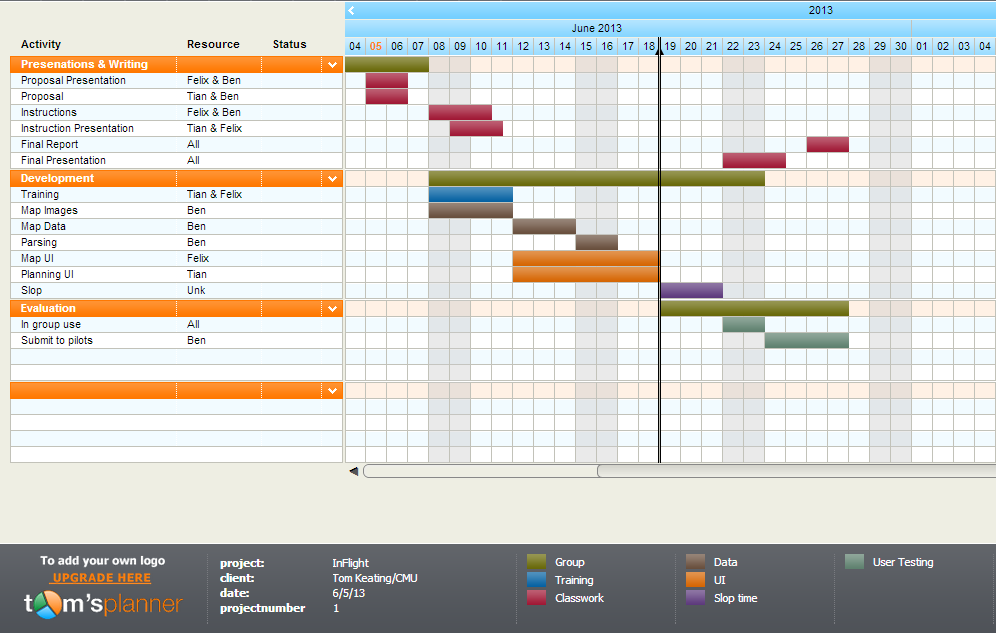
\includegraphics[scale=.4]{gantt}
\caption{Project Timeline Gantt Chart}
\end{figure}
\section{Evaluation}
We intend to use two methods to evaluate our application. The first is traditional user testing, presenting users with the application and asking them to preform a common task. We intend to score this metric based on the amount of time required for the user to find the requested function of the application.

Our second method is centered around pilots. We have access to several instructor pilots with experience using more traditional EFBs and other competitor applications, and can provide actual use cases in real aircraft. We intend this to be the final use case testing, providing a mechanism to find usability issues unique to the airborne environment.

\section{Qualifications}
\begin{itemize}
\item \emph{Benjamin Chung} 
\begin{itemize}
\item Student pilot
\item Junior computer science major
\item Experience with aviation GIS in web applications
\item Multiple internships (Wolfram Research, 2010; Institute for Software Research, 2012, 2013)
\end{itemize}
\end{itemize}
\begin{itemize}
\item \emph{Tianyuan Ding}
\begin{itemize}
\item Sophomore computer science major
\item Experience with C/Java/SML programming
\end{itemize}
\item \emph{Felix Wen}
\begin{itemize}
\item Sophomore mathematics major
\item Experience with C/SML programming language
\end{itemize}
\end{itemize}

\section{Sources}

\begin{enumerate}
\itemsep-1.3em
\item \texttt{ http://developer.android.com/sdk/index.html     } (2013)$\\ $
\item \texttt{  http://maps.google.com/      }(2013)
\end{enumerate} 
\end{document}